% =============================================================================
% Rapport TSPTW — recuit simulé
% Compilation :
%   pdflatex rapport.tex   (deux passes pour la table des matières)
% =============================================================================
\documentclass[11pt,a4paper]{article}

\usepackage[utf8]{inputenc}
\usepackage[T1]{fontenc}
% Si le paquet babel-french est disponible, décommenter la ligne suivante :
% \usepackage[french]{babel}
\usepackage{lmodern}
\usepackage{microtype}

\usepackage[a4paper,margin=2.5cm]{geometry}
\usepackage{amsmath,amssymb}
\usepackage{graphicx}
\usepackage{caption}
\usepackage{enumitem}
\usepackage{xcolor}
\usepackage{fancyhdr}
\usepackage{underscore}  % rend `_` littéral en mode texte
\usepackage{hyperref}

\hypersetup{
  colorlinks=true,
  linkcolor=black,
  urlcolor=blue!50!black,
}

% Dossier des images (les Figure_*.png sont dans image/)
\graphicspath{{image/}}

% En-tête / pied de page
\pagestyle{fancy}
\fancyhf{}
\fancyhead[R]{\itshape\small TSPTW — Recuit simulé}
\fancyfoot[C]{\thepage}
\renewcommand{\headrulewidth}{0pt}

% Espacement plus aéré sur les listes
\setlist[itemize]{itemsep=2pt, topsep=4pt}

% Boîte « insérer ici » pour les figures que l'auteur ajoutera
\newcommand{\figplaceholder}[2]{%
  \begin{figure}[h]
    \centering
    \fbox{\parbox{0.8\linewidth}{\centering\itshape\color{gray}%
      [ insérer ici : #1 ]\\%
      \footnotesize{\rmfamily(remplacer par \texttt{\textbackslash includegraphics[width=...]{#1}})}%
    }}
    \caption{#2}
  \end{figure}%
}

% Titre
\title{\textbf{Recuit simulé pour le TSPTW}\\[6pt]
       \large Implémentation, calibration et analyse expérimentale}
\author{Charles Gaye \and Raphaël Fromager}
\date{Janvier 2026 \\ \small Cours : Complément Parcours Recherche — Info 2}

% =============================================================================
\begin{document}

\maketitle
\thispagestyle{empty}
\vspace{1cm}

\tableofcontents
\newpage

% =============================================================================
\section{Introduction}

Ce rapport présente la démarche et les résultats du projet de métaheuristique consacré
au problème du voyageur de commerce avec contraintes temporelles
(\textsc{TSPTW}, \emph{Travelling Salesman Problem with Time Windows}). On se donne un
ensemble de villes munies de coordonnées planes et d'une fenêtre de visite
$[w_{\text{start}}, w_{\text{end}}]$, et on cherche un ordre de visite, fixant la première
ville et revenant au point de départ, qui minimise la distance totale parcourue tout en
respectant les fenêtres.

Le projet portait sur quatre instances : trois fournies à des fins de mise au point
(de tailles respectives ${\sim}20$, ${\sim}50$ et ${\sim}200$ villes), et une instance
de concours de taille intermédiaire (${\sim}100$ villes). Notre objectif était
d'implémenter et de calibrer un algorithme de recuit simulé, méthode jugée
raisonnable au regard de notre niveau de programmation et bien adaptée aux problèmes
combinatoires de cette taille. L'algorithme de colonie de fourmis avait été envisagé
comme alternative, mais sa mise au point était estimée trop coûteuse en temps de
débogage pour un projet pédagogique.

Ce rapport est volontairement descriptif : il documente les choix faits, ce qu'ils
ont permis d'obtenir, et les limites qui ont été identifiées au cours du travail
(y compris une erreur d'implémentation détectée a posteriori). Il ne vise pas à
présenter une méthode optimisée, et les résultats numériques rapportés sont strictement
ceux qui ont été obtenus pendant le projet.

% =============================================================================
\section{Modélisation et algorithme}

\subsection{Représentation des solutions}

Une solution à une instance de $N$ villes est une permutation des entiers $1, \dots, N$
qui commence par la ville imposée comme dépôt (numérotée $1$ par convention). L'espace
des solutions est ainsi l'ensemble des permutations de $\{2, \dots, N\}$, augmenté du
préfixe $1$, soit $(N-1)!$ éléments. La validité d'une solution dépend du respect des
fenêtres temporelles : on calcule, le long du tour, la date courante d'arrivée à chaque
ville en autorisant l'attente si l'on arrive avant l'ouverture de la fenêtre, et on
compte une violation à chaque fois que la date d'arrivée dépasse la fermeture.

\subsection{Fonction de score}

Faute de pouvoir restreindre rigoureusement la recherche aux solutions admissibles, on
travaille avec une fonction de score pénalisée qui prend la forme :
\begin{equation}
  \mathrm{score}(s) \;=\; \mathrm{distance}(s) \;+\; p_v \, n_{\text{viol}}(s)
                \;+\; p_r \, t_{\text{retard}}(s) \;+\; p_a \, t_{\text{avance}}(s),
  \label{eq:score}
\end{equation}
où $n_{\text{viol}}$ compte les villes visitées hors fenêtre, $t_{\text{retard}}$ est
le retard cumulé en unités de temps et $t_{\text{avance}}$ le temps d'attente cumulé.
Les coefficients $p_v$, $p_r$ et $p_a$ sont des paramètres à calibrer. On notera que
le terme d'avance, par construction, ne pénalise pas la qualité « voyageur » d'une
solution mais traduit plutôt une volonté de regrouper les visites — ce point sera
rediscuté en section~\ref{sec:discussion}.

\subsection{Voisinages}

La fonction de voisinage produit, à partir d'une solution courante, une nouvelle
solution candidate. Un premier essai naïf consistait à appliquer une transposition de
deux villes (sans toucher à la ville $1$). Cette opération s'est révélée trop locale :
sur l'instance la plus simple, l'algorithme convergeait fréquemment vers des solutions
où il satisfaisait les fenêtres temporelles en ne réagençant qu'un petit nombre de
villes, sans réellement explorer l'espace.

Quatre opérateurs ont été retenus, qui agissent sur des blocs contigus :
\begin{itemize}
  \item \texttt{large\_swap} : échange de deux blocs contigus disjoints de même taille.
  \item \texttt{block\_reverse} : inversion de l'ordre dans un bloc.
  \item \texttt{scramble} : permutation uniforme à l'intérieur d'une sous-séquence.
  \item \texttt{insert\_range} : extraction d'un bloc et réinsertion à une autre position.
\end{itemize}

À chaque appel, l'opérateur appliqué est tiré selon un vecteur de probabilité
$p = (p_1, p_2, p_3, p_4)$. En complément, lorsque la solution courante présente au
moins une violation de fenêtre, un opérateur de réparation est tiré $30\,\%$ du temps :
il sélectionne une ville en retard et la réinsère plus tôt dans le tour.

\subsection{Recuit simulé et schéma de refroidissement}

L'algorithme suit le schéma classique : à chaque itération, on tire un voisin $s'$ de
la solution courante $s$, et on l'accepte avec probabilité~$1$ si
$\Delta = \mathrm{score}(s') - \mathrm{score}(s) \le 0$, sinon avec probabilité
$\exp(-\Delta / T)$ (distribution de Gibbs). La température $T$ décroît de manière
géométrique :
\begin{equation}
  T \leftarrow \lambda \, T, \qquad
  \lambda = \left(\frac{T_{\text{end}}}{T_{\text{start}}}\right)^{1/N_{\text{iter}}},
\end{equation}
de sorte que $T$ atteint exactement $T_{\text{end}}$ après $N_{\text{iter}}$ itérations.


\begin{figure}[h]
    \centering
    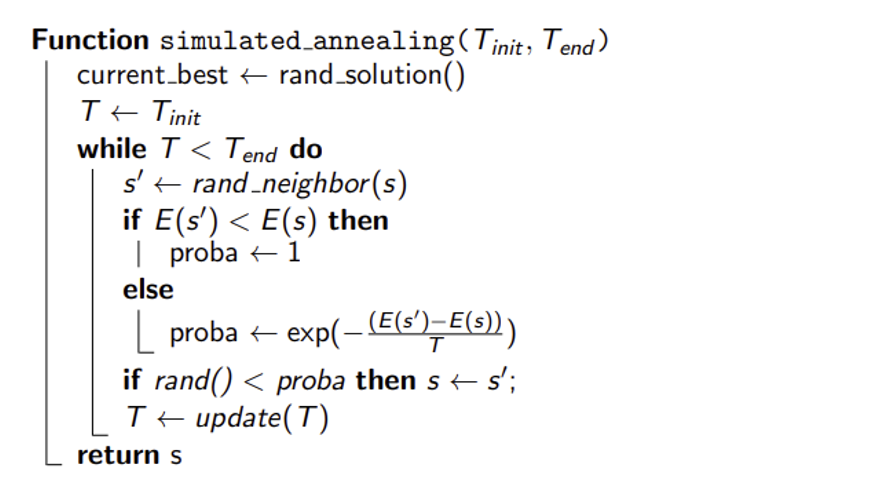
\includegraphics[width=0.8\textwidth]{figures/Figure1.png}
    \caption{Schéma du recuit simulé.}
    \label{fig:sa-scheme}
\end{figure}
% =============================================================================
\section{Implémentation}

Le code est écrit en Python~3 et organisé en modules :
\begin{itemize}
  \item \texttt{io\_utils} — lecture des instances, calcul et mise en cache de la
    matrice de distances avec fermeture pour l'inégalité triangulaire,
    lecture/écriture des fichiers solution.
  \item \texttt{scoring} — fonction de score pénalisée.
  \item \texttt{neighborhoods} — opérateurs de voisinage et heuristique de réparation.
  \item \texttt{sa} — boucle de recuit simulé, paramétrée par une dataclass
    \texttt{SAConfig}.
  \item \texttt{experiments} — moyennage de plusieurs essais et balayages de paramètres.
  \item \texttt{plotting} — tracés de progression et de comparaison avec intervalle
    de confiance.
\end{itemize}

Un point d'entrée \texttt{main\_new.py} expose trois modes d'exécution (un seul recuit,
balayage de probabilités de voisinage, balayage de pénalités) avec une graine aléatoire
optionnelle pour la reproductibilité.

Tâche initialement sous-estimée : le calcul de la matrice de distances avec fermeture
triangulaire est en $\mathcal{O}(N^3)$. Sur l'instance de concours (${\sim}100$ villes),
il est exécuté une seule fois par instance puis mis en cache au format \texttt{.npy},
ce qui rend le coût négligeable pour les expériences répétées.

% =============================================================================
\section{Méthodologie expérimentale}
\label{sec:methodo}

Pour comparer deux paramétrages, exécuter un seul recuit ne suffit pas : la variance
entre essais peut masquer ou simuler des écarts de performance. On a mis en place une
procédure de moyennage qui consiste à exécuter, pour chaque configuration,
$n_{\text{runs}}$ recuits indépendants et à empiler les courbes du meilleur score
atteint au fil des itérations.

Le score affiché dans les comparaisons est calculé sous une métrique de référence
\emph{indépendante} du paramétrage testé (pénalités fixées à $p_v = 500$, $p_r = 25$,
$p_a = 3$). Cela permet de comparer entre eux des recuits qui auraient utilisé des
pénalités différentes pour piloter leur trajectoire, sans que la métrique d'évaluation
soit elle-même sensible au paramétrage.

On reporte la moyenne et un intervalle de confiance à $95\,\%$ autour de cette moyenne,
calculé en supposant les essais indépendants et identiquement distribués :
\begin{equation}
  \mathrm{IC} \;=\; \overline{X} \;\pm\; 1{.}96 \, \frac{\sigma}{\sqrt{n_{\text{runs}}}}.
\end{equation}
Cet IC borne la moyenne d'\emph{une} configuration à un instant donné ; il ne quantifie
pas la variabilité d'un essai isolé. Cette nuance jouera un rôle dans la
discussion (section~\ref{sec:discussion}).

\begin{figure}[h]
    \centering
    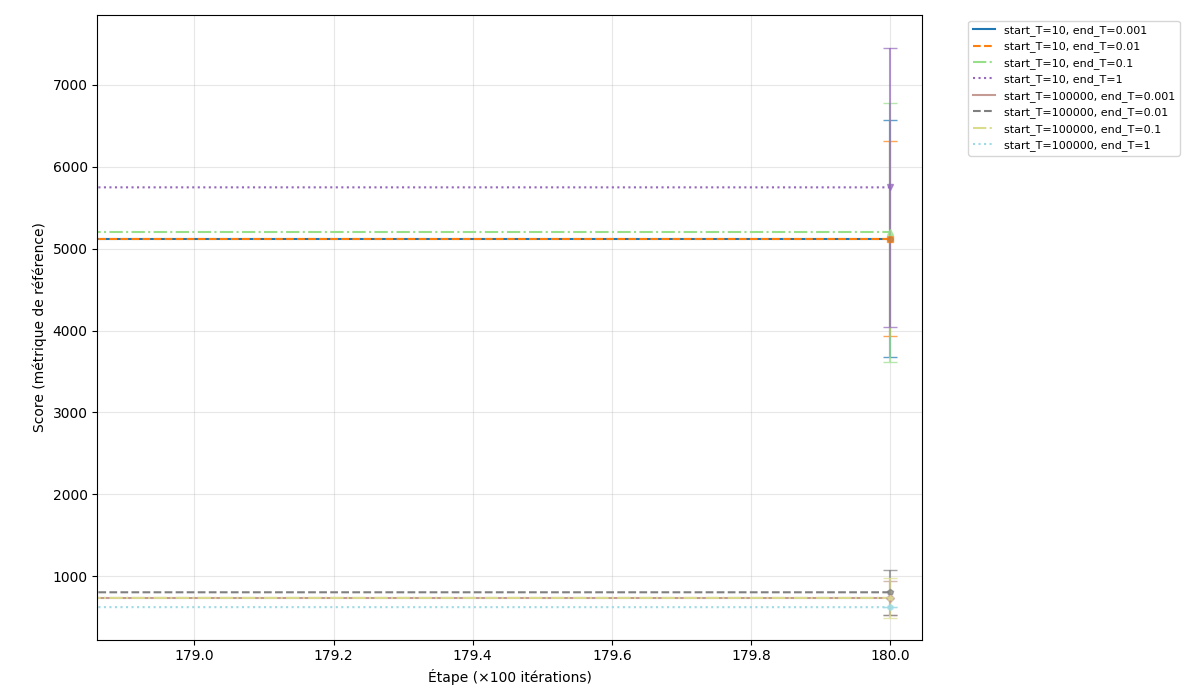
\includegraphics[width=0.8\textwidth]{figures/Figure4.png}
    \caption{Premier balayage de la température initiale.}
    \label{fig:sweep-tstart}
\end{figure}


% =============================================================================
\section{Résultats}
\label{sec:resultats}

\subsection{Calibration des températures}

Les premières valeurs essayées ($T_{\text{start}} \approx 100$, $T_{\text{end}} \approx 0{.}01$,
environ $5\,000$ itérations) ne permettaient pas de trouver de solution admissible. Le
diagnostic, posé après une discussion en cours, a été que ces paramètres faisaient
décroître la température trop vite : la probabilité d'accepter un voisin de moins bonne
qualité devenait rapidement négligeable, et l'algorithme se comportait en pratique
comme une descente locale dès les premières itérations.

En relevant la température initiale dans la plage $[10^4, 10^5]$ et en augmentant le
nombre d'itérations à environ $50\,000$, l'algorithme a commencé à produire des
solutions sans retard sur l'instance~1. Un balayage exponentiel de $T_{\text{start}}$
sur $[10^3, 10^6]$, affiné progressivement, a conduit à retenir
$T_{\text{start}} = 5\,000$ comme valeur usuelle. La température finale s'est révélée
plus difficile à fixer : nous avons constaté empiriquement qu'une valeur plus faible
était nécessaire pour les instances comportant davantage de villes ($\approx 1$ pour
l'instance~1, $\approx 0{.}05$--$0{.}5$ pour les instances~2 et~3, $\approx 0{.}1$
retenu pour l'instance de concours, qui est de taille intermédiaire). Cette dépendance
n'a pas été quantifiée par une expérience dédiée.


\begin{figure}[h]
    \centering
    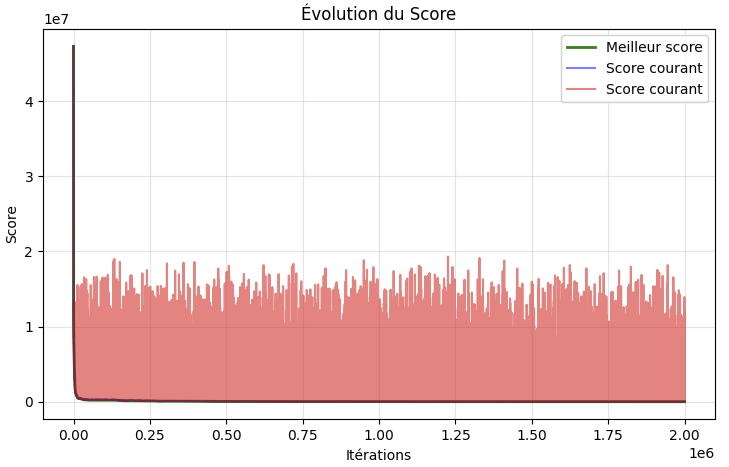
\includegraphics[width=0.8\textwidth]{figures/Figure2.png}
    \caption{Évolution typique du score au cours d'un recuit (instance 3).}
    \label{fig:score-graph}
\end{figure}

\begin{figure}[h]
    \centering
    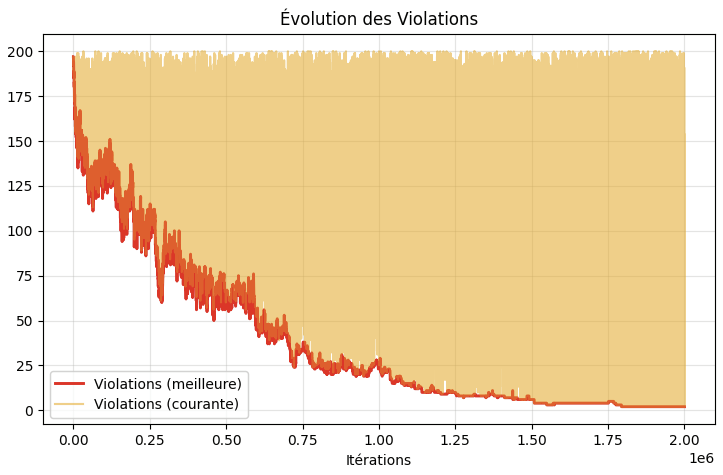
\includegraphics[width=0.8\textwidth]{figures/Figure3.png}
    \caption{Évolution typique du nombre de violations (instance 3).}
    \label{fig:violation-graph}
\end{figure}

\subsection{Choix du voisinage}

L'effet du vecteur $p$ de probabilités de voisinage a été étudié en plusieurs étapes.
Une première comparaison entre les vecteurs unitaires $e_1, e_2, e_3, e_4$ (un seul
opérateur actif) a fait ressortir \texttt{scramble} (i.e.\ $e_3$) comme le plus
performant. Des combinaisons à dominante $e_3$ (par exemple $p = (0,\, 0{.}1,\, 0{.}75,\, 0{.}15)$)
ont donné des résultats comparables au $e_3$ pur, sans qu'on ait pu mettre en évidence
de combinaison strictement meilleure : tous les vecteurs testés à dominante
\texttt{scramble} produisaient des courbes dont les intervalles de confiance se
chevauchaient.

Les vecteurs retenus pour la suite étaient donc $p = (0, 0, 1, 0)$ et
$p = (0, 0{.}1, 0{.}8, 0{.}1)$, ainsi que des variantes proches.


\begin{figure}[h]
    \centering
    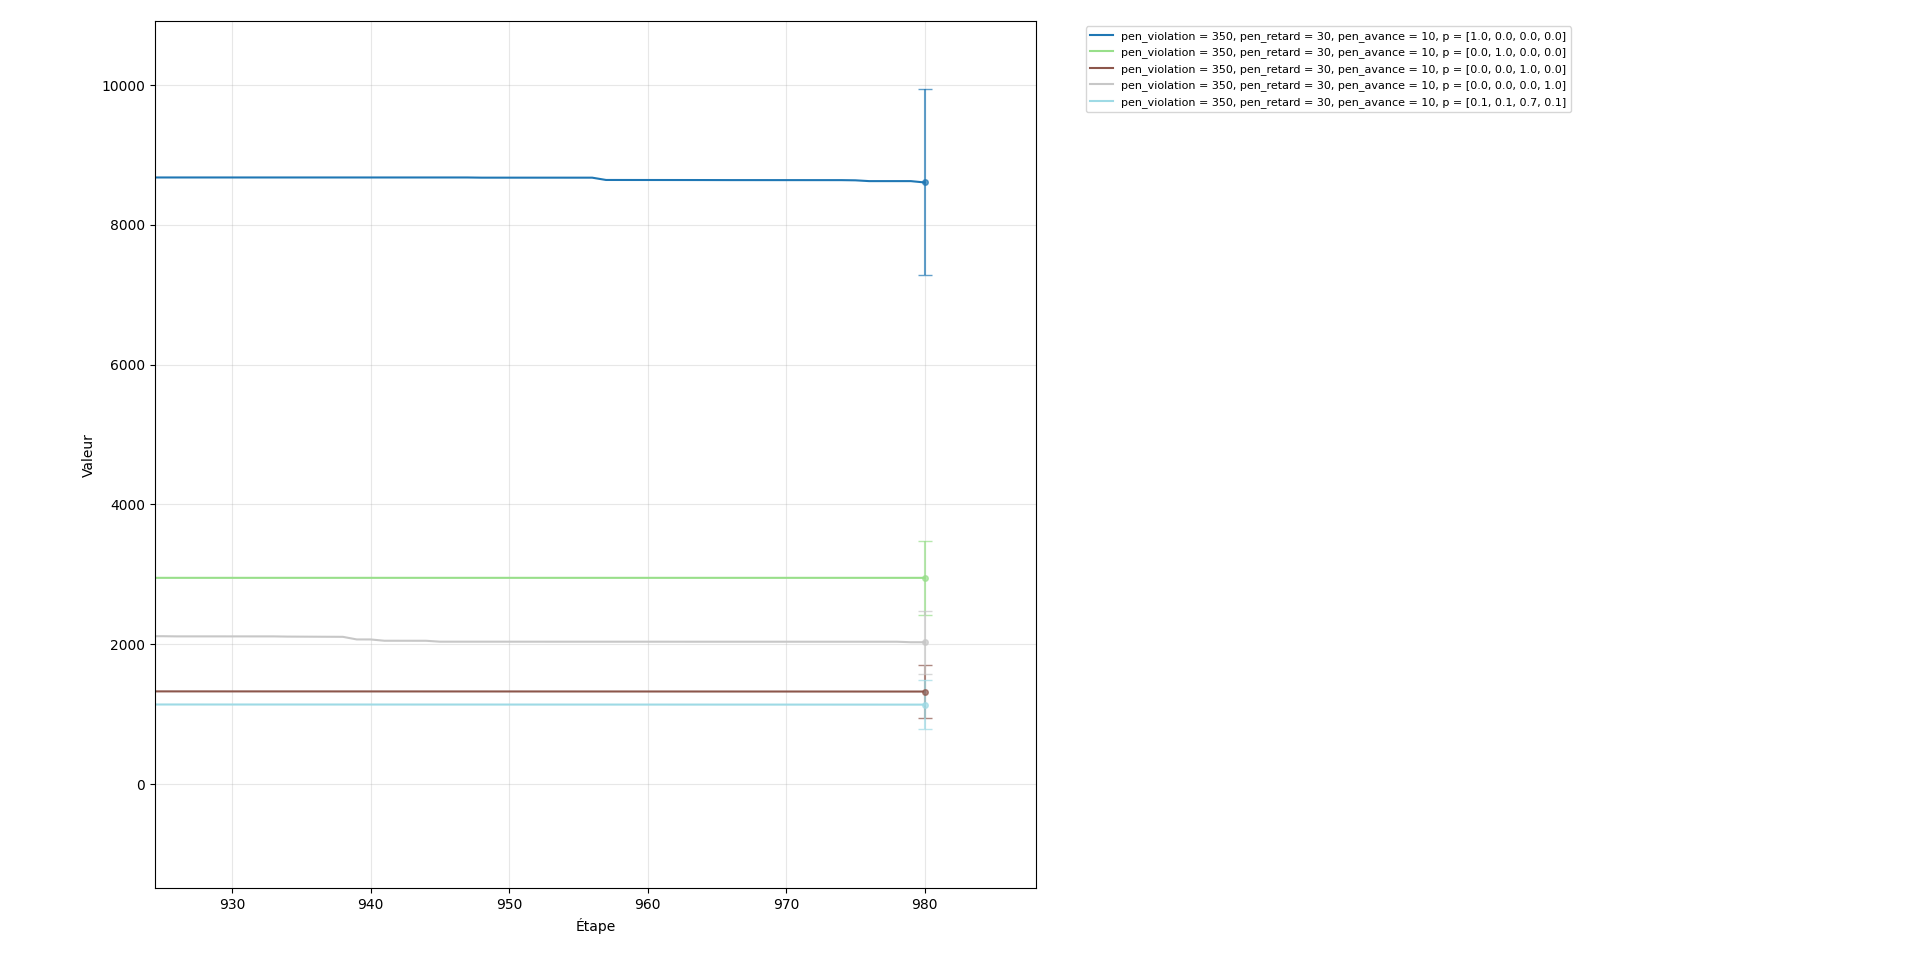
\includegraphics[width=0.8\textwidth]{figures/Figure5.png}
    \caption{Comparaison des vecteurs unitaires et d'un vecteur à dominante \texttt{scramble}.}
    \label{fig:unit-vs-scramble}
\end{figure}


\begin{figure}[h]
    \centering
    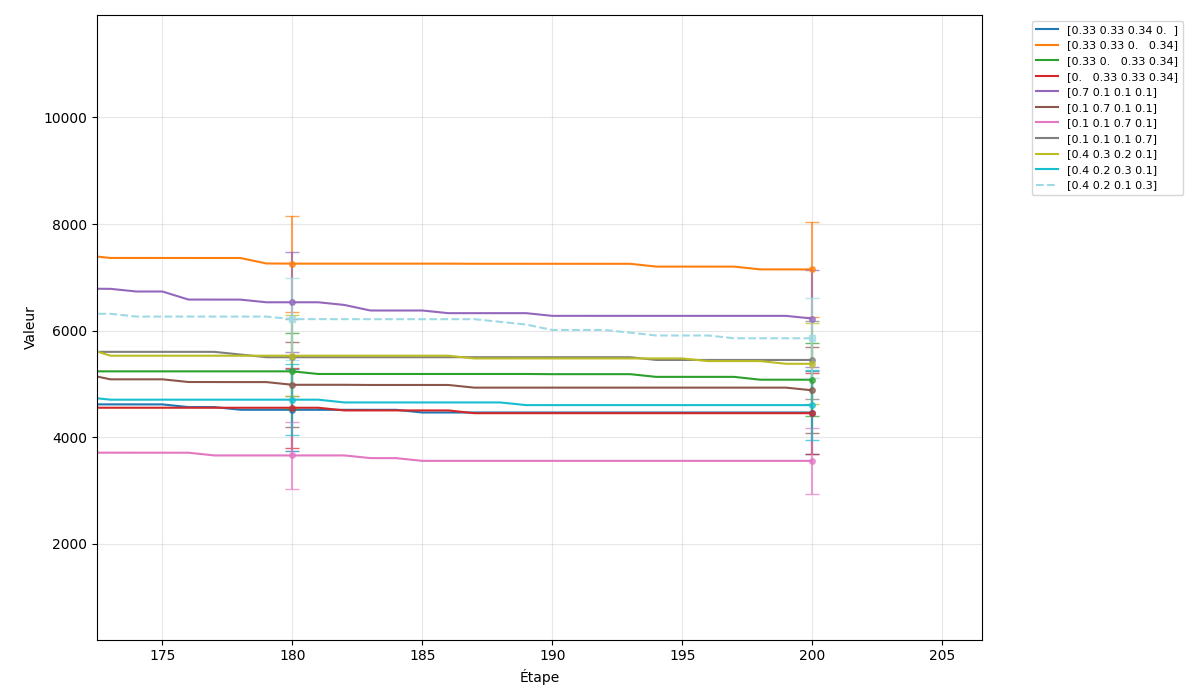
\includegraphics[width=0.8\textwidth]{figures/Figure6.png}
    \caption{Comparaison de plusieurs vecteurs à dominante \texttt{scramble}.}
    \label{fig:full-scrumble}
\end{figure}

\subsection{Pénalités}

La fonction de score retenue après calibration est :
\begin{equation}
  \mathrm{score} \;=\; \mathrm{distance} \;+\; 350 \, n_{\text{viol}}
                 \;+\; 30 \, t_{\text{retard}} \;+\; 10 \, t_{\text{avance}}.
\end{equation}
Le coefficient $350$ sur les violations a été abaissé par rapport à la valeur initiale
($10\,000$) pour ne pas écraser les autres termes : avec une pénalité trop forte,
l'algorithme pouvait satisfaire toutes les fenêtres en restant sur des solutions de
mauvaise qualité au sens de la distance.

\begin{figure}[h]
    \centering
    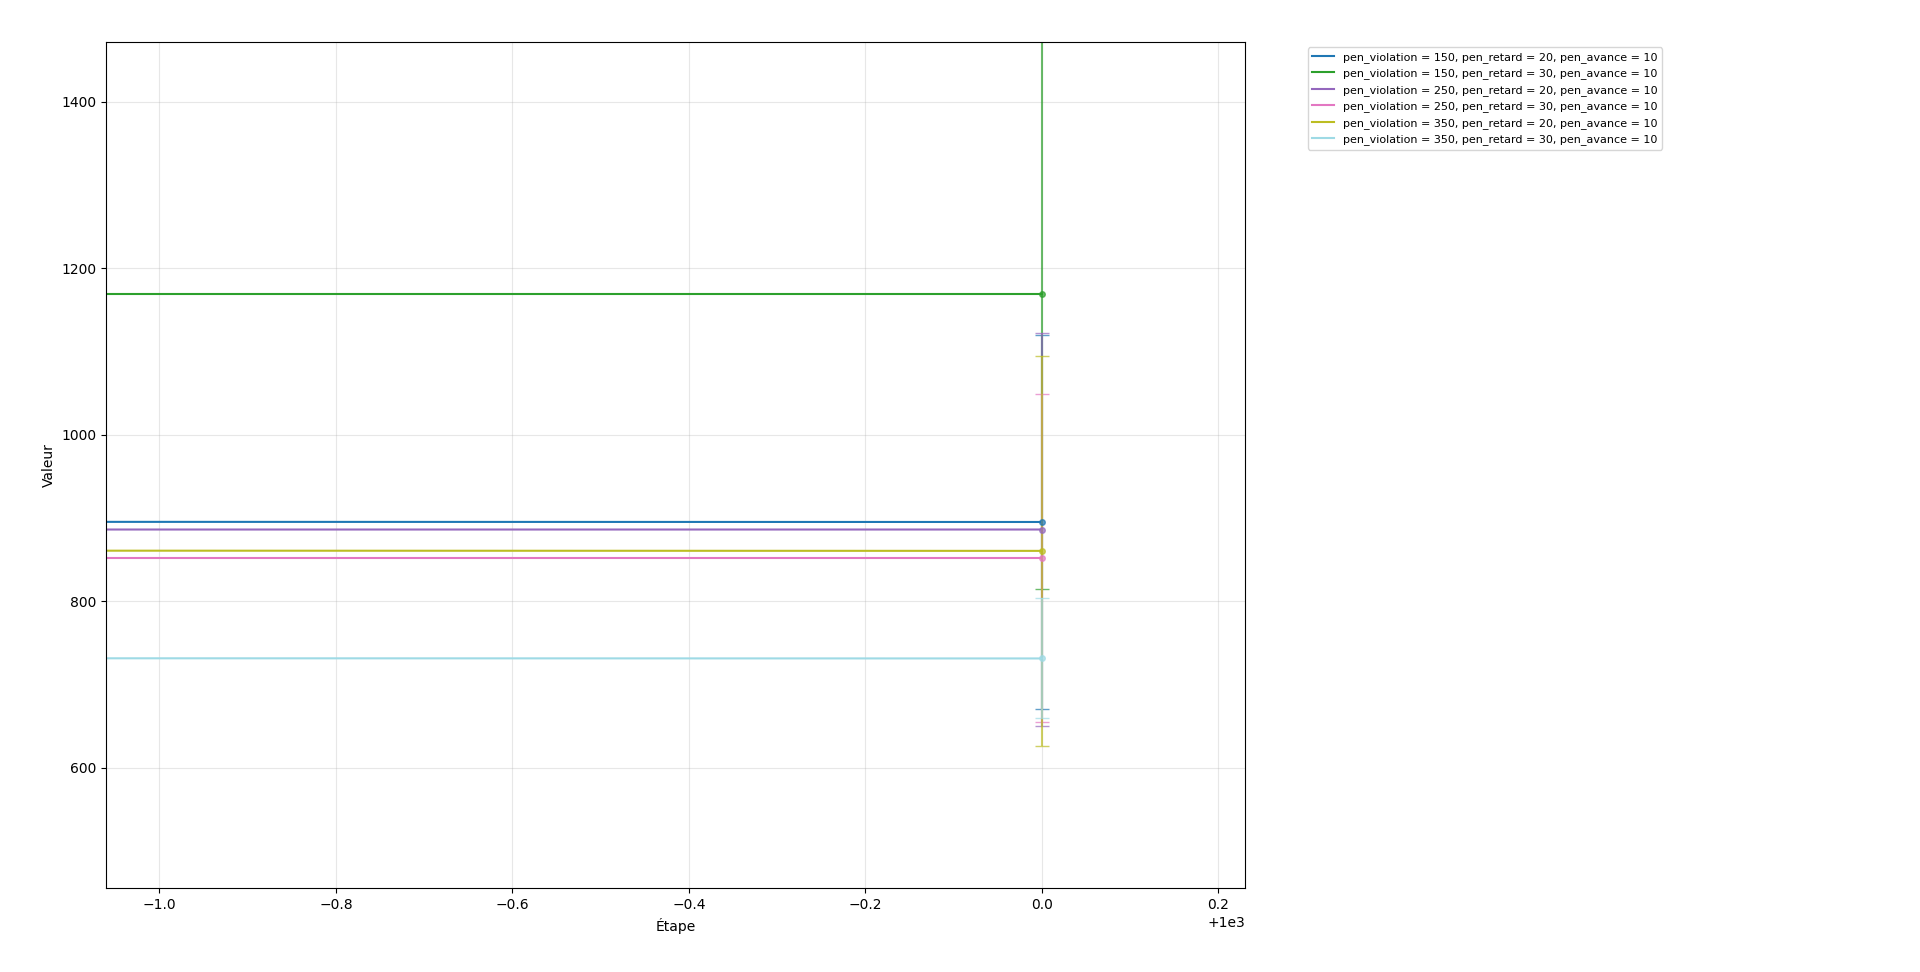
\includegraphics[width=0.8\textwidth]{figures/Figure7.png}
    \caption{Exemple de comparaison sur les pénalités.}
    \label{fig:pen-comparison}
\end{figure}

Un effet a été observé sur le coefficient d'avance : le groupe avec $p_a = 10$ obtenait,
sur l'instance de concours, une moyenne finale plus basse que le groupe avec $p_a = 5$,
avec des intervalles de confiance qui se chevauchaient peu (cf.\ figure suivante).
Ce point est rediscuté en section~\ref{ssec:bug-avance}.

\begin{figure}[h]
    \centering
    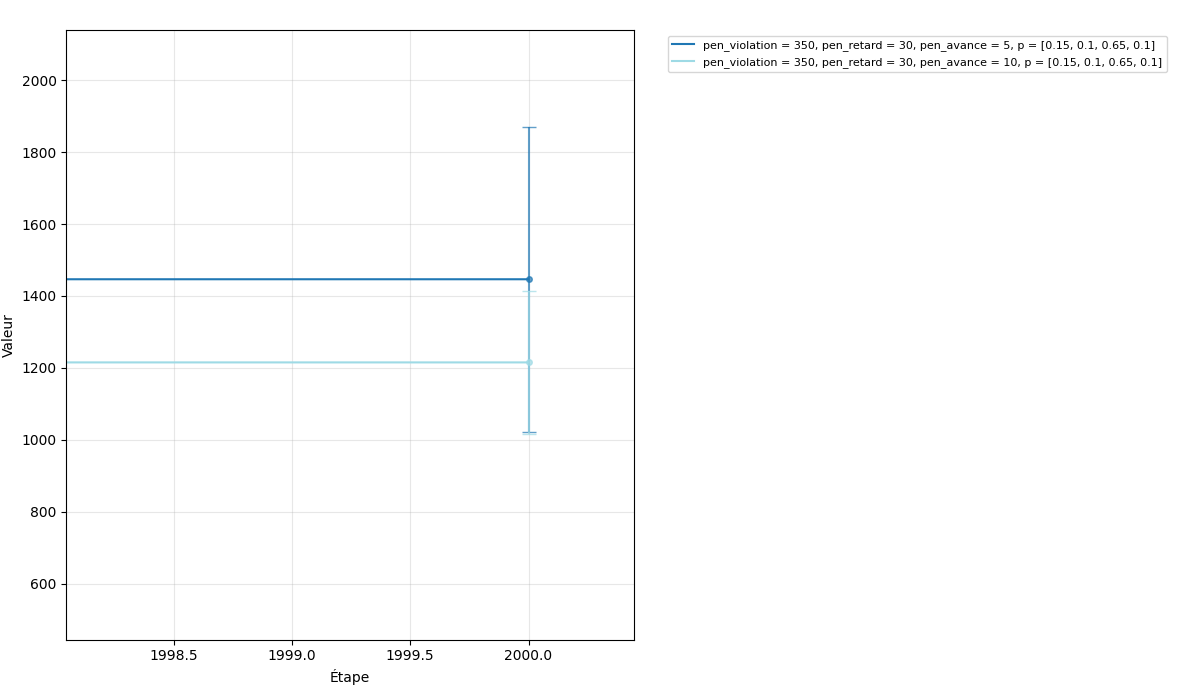
\includegraphics[width=0.8\textwidth]{figures/Figure8.png}
    \caption{Comparaison des scores finaux pour $p_a = 5$ et $p_a = 10$, autres paramètres égaux.}
    \label{fig:pena-comparison}
\end{figure}

\subsection{Résultats par instance}

Avec le paramétrage final ($T_{\text{start}} = 5\,000$, $T_{\text{end}} \approx 0{.}1$,
de $10^5$ à $2 \times 10^6$ itérations selon l'instance, $p$ à dominante
\texttt{scramble}, pénalités $(350, 30, 10)$) :

\begin{itemize}
  \item \textbf{Instance 1} (${\sim}20$ villes) : la solution optimale donnée avec le
    sujet est retrouvée systématiquement dès le premier essai pour un nombre
    d'itérations suffisant.
  \item \textbf{Instance 2} (${\sim}50$ villes) : la solution optimale est retrouvée.
  \item \textbf{Instance 3} (${\sim}200$ villes) : aucune solution admissible n'a été
    trouvée. Les meilleurs essais présentent encore $2$ à $3$ villes en retard.
  \item \textbf{Instance de concours} (${\sim}100$ villes) : une solution admissible
    (sans avance ni retard) est trouvée sans difficulté ; en revanche, le score varie
    d'un essai à l'autre, ce qui suggère que la solution ainsi obtenue n'est pas
    systématiquement optimale.
\end{itemize}


\begin{figure}[h]
    \centering
    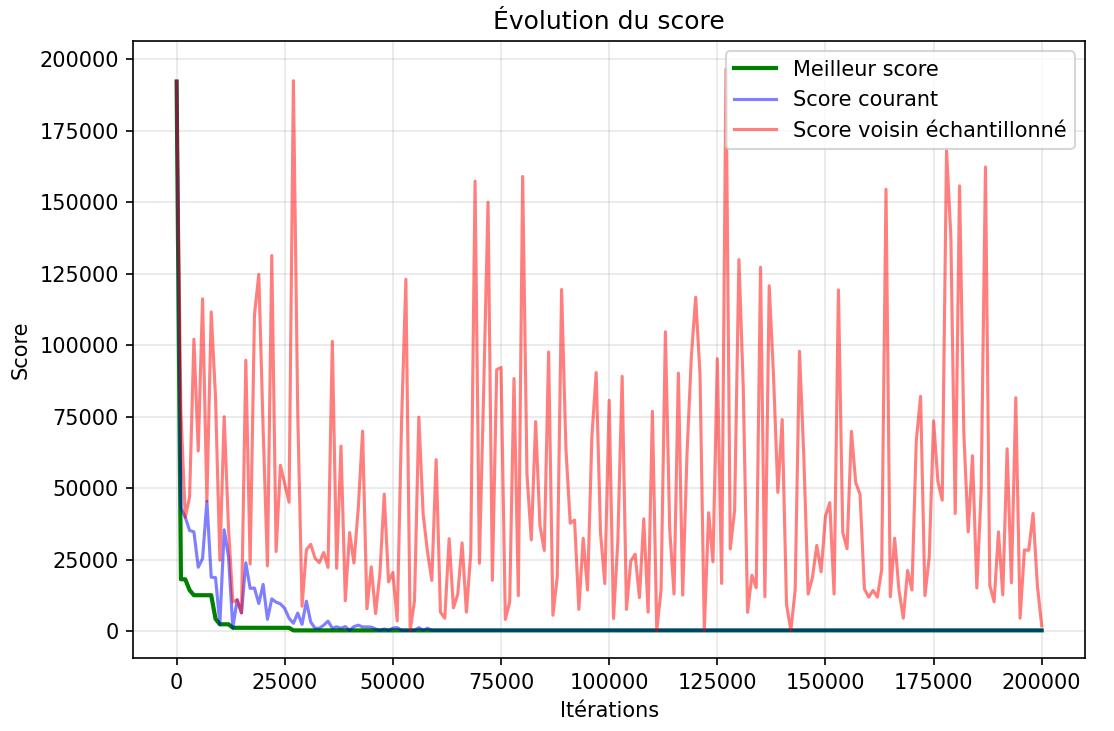
\includegraphics[width=0.8\textwidth]{figures/Figure9.png}
    \caption{Recuit ayant atteint la solution optimale sur l'instance 1.}
    \label{fig:best-1}
\end{figure}

\begin{figure}[h]
    \centering
    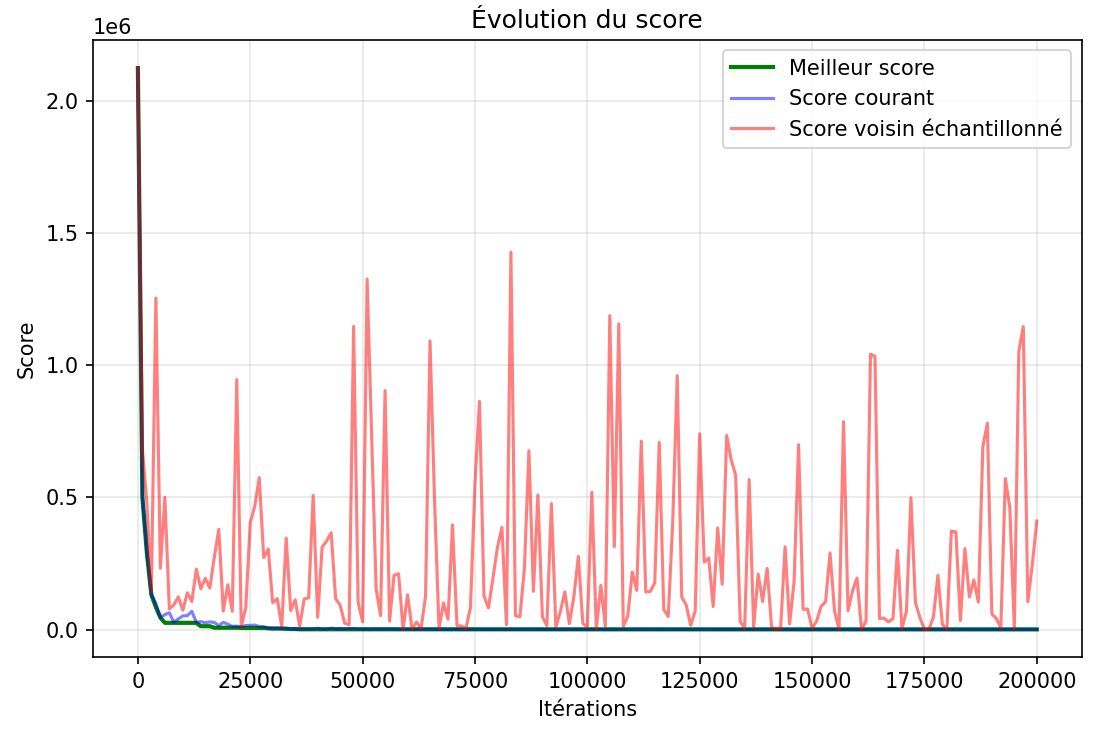
\includegraphics[width=0.8\textwidth]{figures/Figure10.png}
    \caption{Recuit ayant atteint la solution optimale sur l'instance 2.}
    \label{fig:best-2}
\end{figure}

\begin{figure}[h]
    \centering
    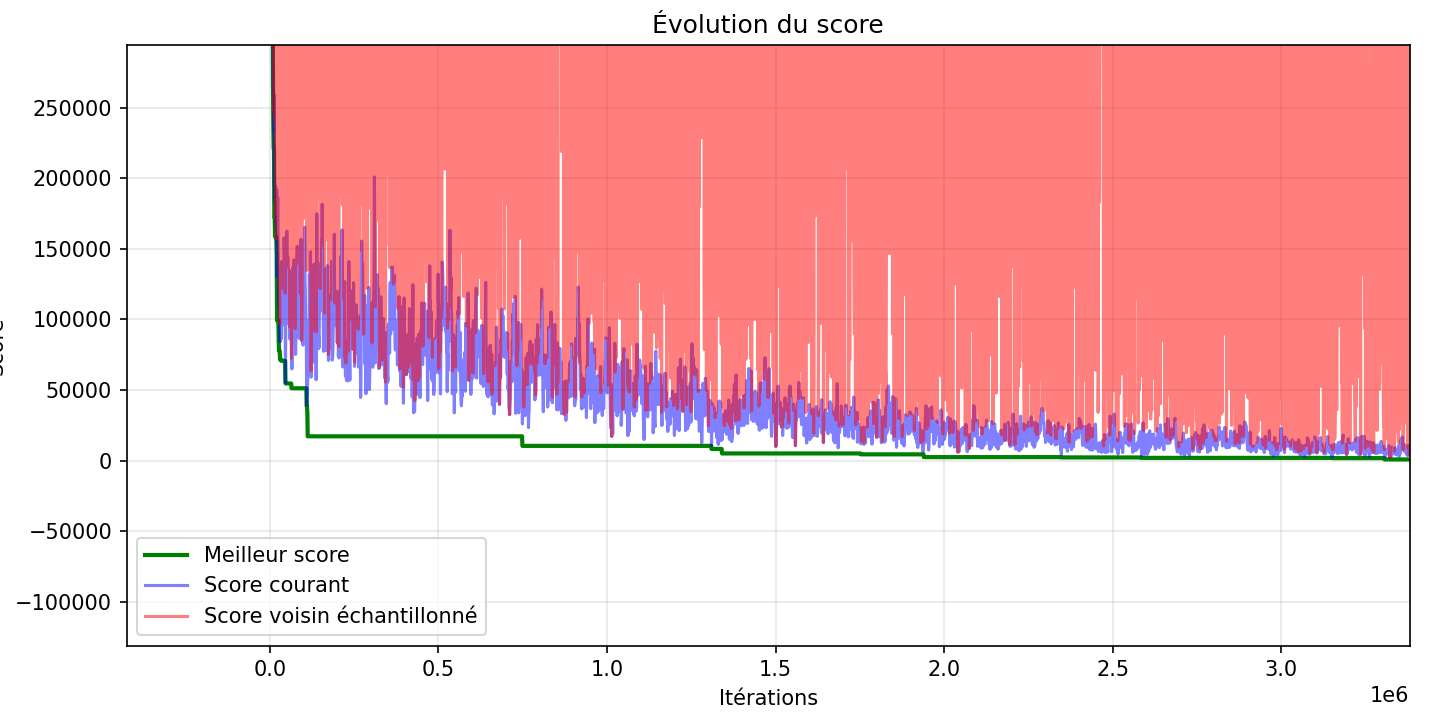
\includegraphics[width=0.8\textwidth]{figures/Figure11.png}
    \caption{Zoom sur le recuit ayant atteint la solution optimale sur l'instance 3.}
    \label{fig:best-3}
\end{figure}

\begin{figure}[h]
    \centering
    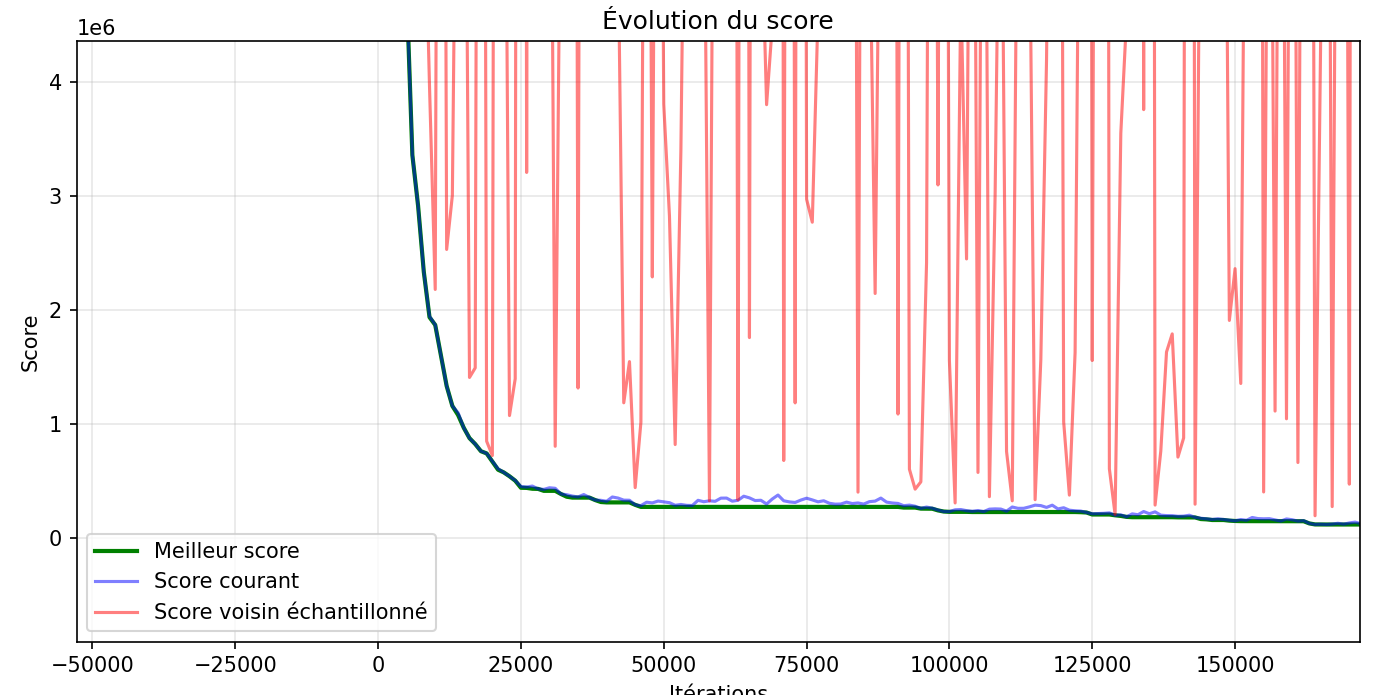
\includegraphics[width=0.8\textwidth]{figures/Figure12.png}
    \caption{Zoom sur le recuit ayant atteint la solution optimale sur l'instance concours.}
    \label{fig:best-concours}
\end{figure}

Nous savons depuis la fin du projet que l'instance de concours dispose d'une solution
optimale publiquement connue, dont le score est sensiblement meilleur que celui que
nous rapportons. Nous indiquons ce fait par souci d'honnêteté ; nous n'avons pas
réalisé de comparaison chiffrée a posteriori car notre travail est resté dans le
périmètre des essais effectués pendant le projet.

% =============================================================================
\section{Discussion et limites}
\label{sec:discussion}

\subsection{Erreur d'implémentation sur la pénalité d'avance}
\label{ssec:bug-avance}

En relisant la fonction de score après le rendu, nous avons identifié une erreur dans
le calcul de l'avance. L'extrait en cause est le suivant :
\begin{verbatim}
if duree < next_start:
    duree = next_start          # <-- duree écrasée d'abord
    avance += next_start - duree  # <-- vaut donc 0
\end{verbatim}
Après l'affectation \texttt{duree = next\_start}, la quantité
\texttt{next\_start - duree} vaut $0$. La variable $t_{\text{avance}}$ est donc
systématiquement nulle, et le terme $p_a \cdot t_{\text{avance}}$ ne contribue jamais
au score. À paramétrage par ailleurs égal et à graine aléatoire fixée, le recuit
produit la \emph{même trajectoire} pour toute valeur de $p_a$ — ce que nous avons
vérifié a posteriori sur le code restructuré.

Cette erreur soulève une question : pourquoi la figure relative à $p_a$ fait-elle
apparaître un écart entre les groupes $p_a = 5$ et $p_a = 10$, alors que l'algorithme,
théoriquement, ne devrait pas distinguer ces deux configurations~?

L'explication la plus plausible tient à la méthodologie de comparaison plutôt qu'à un
effet réel de $p_a$ :
\begin{itemize}
  \item Les deux configurations comparées dans une même session de balayage partagent
    l'état global de \texttt{np.random} : la première configuration consomme une
    portion de la séquence aléatoire, la deuxième commence là où la première s'est
    arrêtée. Les deux groupes ne voient donc pas les mêmes graines, et la comparaison
    n'isole pas l'effet de $p_a$.
  \item L'intervalle de confiance affiché borne la moyenne d'une configuration à
    partir de la variance des essais qu'elle contient. Il ne reflète pas la
    variabilité induite par le choix de la séquence aléatoire entre configurations.
    L'écart visible entre les deux moyennes peut donc être plus large que ne le
    laisse entendre la séparation des intervalles.
\end{itemize}

Ces deux points combinés sont compatibles avec l'écart observé. Une comparaison plus
rigoureuse nécessiterait de fixer une graine par essai, partagée entre configurations,
ce qui n'a pas été fait dans le projet et que nous n'avons pas refait depuis. Le code
restructuré expose désormais un argument \texttt{rng\_seed} permettant ce type de
protocole.

\subsection{Coefficient sur les violations}

Le passage de $p_v = 10\,000$ à $p_v = 350$ a clairement amélioré la capacité de
l'algorithme à explorer des solutions de meilleure qualité une fois les fenêtres
satisfaites. Au-delà de ce constat qualitatif, nous n'avons pas conduit d'étude
systématique de l'effet de $p_v$ sur l'instance de concours.

\subsection{Limites de la fonction de voisinage}

Sur l'instance~3, l'algorithme stagne avec $2$ à $3$ violations résiduelles. Nous
pensons qu'une fonction de voisinage informée par l'état courant — par exemple un
opérateur qui choisit la position de réinsertion en fonction des fenêtres temporelles
plutôt qu'aléatoirement — aurait été nécessaire pour franchir ce palier. Nous n'avons
pas eu le temps de la mettre en œuvre.

\subsection{Écart à l'optimum sur l'instance de concours}

Plusieurs facteurs peuvent expliquer l'écart entre notre meilleur score et l'optimum
publiquement connu :
\begin{itemize}
  \item Une intensification insuffisante en fin de recuit : la température finale et
    la longueur de la phase de basse température n'ont pas été calibrées
    spécifiquement pour cette instance.
  \item Un voisinage non spécialisé pour l'aspect temporel : nos quatre opérateurs
    travaillent sur la structure de permutation sans tenir compte des fenêtres.
  \item Le bug d'avance : la pénalité d'avance ne contribuant pas au score,
    l'algorithme n'avait pas d'incitation à regrouper les visites compatibles, ce qui
    aurait pu favoriser des tours plus courts dans la phase d'intensification.
  \item Le choix de la graine et la dispersion entre essais : un nombre limité
    d'essais sur l'instance de concours a pu masquer des solutions meilleures
    atteignables avec une autre initialisation.
\end{itemize}

% =============================================================================
\section{Conclusion}

Le projet a permis d'implémenter et de calibrer un recuit simulé pour le \textsc{TSPTW}.
Sur les instances~1 et~2, l'algorithme retrouve la solution optimale fournie. Sur
l'instance~3 il atteint des solutions admissibles et presque admissible mais les scores finaux restent très élevé, même  Sur l'instance de concours il produit une solution admissible dont
nous ne pouvons pas garantir l'optimalité, et nous savons depuis la fin du projet
qu'une meilleure solution existe.

Au-delà des résultats, le projet a mis en évidence des points méthodologiques
importants : la nécessité de calibrer la température en cohérence avec le nombre
d'itérations, la limite des comparaisons par moyennage lorsque l'état aléatoire
n'est pas contrôlé, et le coût d'une erreur d'implémentation discrète comme celle que
nous avons identifiée a posteriori sur la pénalité d'avance. Le code a été restructuré
en modules pour permettre des reprises ultérieures, et expose désormais un argument
de graine pour faciliter les comparaisons rigoureuses.

\end{document}
